\chapter{Генераторы псевдослучайных чисел}\label{chapter-generators}
\selectlanguage{russian}

Для работы многих криптографических примитивов необходимо уметь получать случайные числа:
\begin{itemize}
	\item вектор инициализации для отдельных режимов сцепления блоков должен быть случайным числом (см. раздел~\ref{section-block-chaining});
	\item для генерации пар открытых и закрытых ключей необходимы случайные числа (см. главу~\ref{chapter-public-key});
	\item стойкость многих протоколов распределения ключей (см. главу~\ref{chapter-key-distribution-protocols}) основывается в том числе на выработке случайных чисел (\langen{nonce}), которые не может предугадать злоумышленник.
\end{itemize}

Генератором случайных чисел (\langen{random number generator})\index{генератор!случайных чисел} мы будем называть процесс\footnote{Есть и строгое математическое определение генератора в общем смысле. Генератором называется функция $g: \left\{0, 1\right\}^{n} \to \left\{0, 1\right\}^{q\left(n\right)}$, вычислимая за полиномиальное время. Однако мы пока не будем использовать это определение, чтобы показать разницу между истинно случайными числами и псевдослучайными.}, результатом работы которого является случайная последовательность чисел, а именно такая, что зная произвольное число предыдущих чисел последовательности (и способ их получения), даже теоретически нельзя предсказать следующее с вероятностью больше заданной. К таким случайным процессам можно отнести:

\begin{itemize}
	\item результат работы счётчика элементарных частиц, работа с которым включена в лабораторный практикум по общей физике для студентов первого курса МФТИ;
	\item время между нажатиями клавиш на клавиатуре персонального компьютера или расстояние, которое проходит <<мышь>> во время движения;
	\item время между двумя пакетами, полученными сетевой картой;
	\item тепловой шум, измеряемый звуковой картой на входе аналогового микрофона, даже при отсутствии самого микрофона.
\end{itemize}

Хотя для всех этих процессов можно предсказать приблизительное значение (чётное или нечётное), его последний бит будет оставаться достаточно случайным для практических целей. С учётом данной поправки их можно называть надёжными или качественными генераторами случайных чисел.

Однако к генератору случайных чисел предъявляются и другие требования. Кроме уже указанного критерия \emph{качественности} или \emph{надёжности}, генератор должен быть \emph{быстрым} и \emph{дешёвым}. Быстрым -- чтобы получить большой объём случайной информации за заданный период времени. И дешёвым -- чтобы его можно было бы использовать на практике. Количество случайной информации от перечисленных выше генераторов составляет не более десятков килобайт в секунду (для теплового шума) и значительно меньше, если мы будем требовать ещё и равномерность распределения полученных случайных чисел.

С целью получения большего объёма случайной информации используют специальные алгоритмы, которые называют генераторами псевдослучайных чисел (ГПСЧ). ГПСЧ -- это детерминированный алгоритм, выходом которого является последовательность чисел, обладающая свойством случайности. Работу ГПСЧ можно описать следующей моделью. На подготовительном этапе оперативная память, используемая алгоритмом, заполняется начальным значением (\langen{seed}). Далее на каждой итерации своей работы ГПСЧ выдаёт на выход число, которое является функцией от состояния оперативной памяти алгоритма, и меняет содержимое своей памяти по определённым правилам. Содержимое оперативной памяти называется \emph{внутренним состоянием} генератора.

Как и у любого алгоритма, у ГПСЧ есть определённый размер используемой оперативной памяти\footnote{Только алгоритмы с фиксированным размером используемой оперативной памяти и можно называть \emph{генераторами} в строгом математическом смысле этого слова, как следует из определения.}. Исходя из практических требований, предполагается, что размер оперативной памяти для ГПСЧ сильно ограничен. Так как память алгоритма ограничена, то ограничено и число различных внутренних состояний алгоритма. В силу того что выдаваемые ГПСЧ числа являются функцией от внутреннего состояния, то любой ГПСЧ, работающий с ограниченным размером оперативной памяти и не принимающий извне дополнительной информации, будет иметь \emph{период}. Для генератора с памятью в $n$ бит максимальный период, очевидно, равен $2^n$.

Качество детерминированного алгоритма, то есть то, насколько полученная последовательность обладает свойством случайной, можно оценить с помощью тестов, таких как набор тестов NIST (\langen{National Institute of Standards and Technology}, США,~\cite{NIST:2001}). Данный набор содержит большое число различных проверок, включая частотные тесты бит и блоков, тесты максимальных последовательностей в блоке, тесты матриц и так далее.

\section{Линейный конгруэнтный генератор}\label{section-linear-congruential-generator}\index{генератор!линейный конгруэнтный}
\selectlanguage{russian}

Алгоритм был предложен Лемером (\langen{Derrick Henry Lehmer},~\cite{Lehmer:1951:1, Lehmer:1951:2}) в 1949 году. Линейный конгруэнтный генератор основывается на вычислении последовательности $x_n, x_{n+1}, \dots$, такой что:
	\[x_{n+1} = a \cdot x_n + c \mod m.\]

Числа $a, c, m$, $ 0 < a < m, 0 < c < m$ являются параметрами алгоритма.

\example
Для параметров $a = 2, c = 3, m = 5$ и начального состояния $x_0 = 1$ получаем последовательность: $0, 3, 4, 0, 3, 4, \dots$
\exampleend

Максимальный период ограничен значением $m$. Но максимум периода достигается тогда и только тогда, когда~\cite[Линейный конгруэнтный метод]{Knuth:2001:2}:

\begin{itemize}
	\item числа $c$ и $m$ взаимно просты\index{числа!взаимно простые};
	\item число $a - 1$ кратно каждому простому делителю числа $m$;
	\item число $a - 1$ кратно 4, если $m$ кратно 4.
\end{itemize}

Конкретная реализация алгоритма может использовать в качестве выхода либо внутреннее состояние целиком (число $x_n$), либо его отдельные биты. Линейный конгруэнтный генератор является простым (то есть <<дешёвым>>) и быстрым генератором, результатом его работы является статистически качественная псевдослучайная последовательность. Линейный конгруэнтный генератор нашёл широкое применение в качестве стандартной реализации функции \texttt{random} в различных компиляторах и библиотеках времени исполнения (см. таблицу~\ref{table:lcg}). Но, забегая вперёд, его использование в криптографии недопустимо. Зная два последовательных значения выхода генератора ($x_n$ и $x_{n+1}$) и единственный параметр схемы $m$, можно решить систему уравнений и найти $a$ и $c$, чего будет достаточно для нахождения всей дальнейшей (или предыдущей) части последовательности. Параметр $m$, в свою очередь, можно найти перебором, начиная с некоторого $\min(X): X \geq x_i$, где $x_i$ -- наблюдаемые элементы последовательности.

\begin{landscape}
{\renewcommand{\arraystretch}{1.5}
\begin{table}[h]
\begin{tabular}{|p{0.34\linewidth}|r|r|r|l|}
\hline
									& a		& c		& m		& используемые биты	\\
\hline
\cite{Press:2007}~Numerical Recipes: The Art of Scientific Computing	& 1664525	& 1013904223	& $2^{32}$	& 			\\
\cite{Knuth:2005}~MMIX in The Art of Computer Programming & \tiny{6364136223846793005} & \tiny{1442695040888963407}	& $2^{64}$	&	\\
\hline
\cite{Entacher:1997}~ANSI C:
\tiny{(Watcom, Digital Mars, CodeWarrior, IBM VisualAge C/C++)}		& 1103515245	& 12345		& $2^{31}$	& биты с 30 по 16-й	\\
\cite{Sirca:Horvat:2012}~glibc						& 1103515245	& 12345		& $2^{31}$	& биты с 30 по 0-й	\\
C99, C11 (ISO/IEC 9899) 						& 1103515245	& 12345		& $2^{32}$	& биты с 30 по 16-й	\\
C++11 (ISO/IEC 14882:2011) 						& 16807		& 0		& $2^{31} - 1$	& 			\\
Apple CarbonLib             			                       	& 16807		& 0		& $2^{31} - 1$	& 			\\
Microsoft Visual/Quick C/C++                                    	& 214013	& 2531011	& $2^{32}$	& биты с 30 по 16-й	\\
\hline
\cite{Bucknall:2001}~Borland Delphi					& 134775813	& 1		& $2^{32}$	& \\
\cite{MS-VBRAND:2004}~Microsoft Visual Basic \tiny{(версии 1--6)}	& 1140671485	& 12820163	& $2^{24}$	& 			\\
\cite{Mak:2003}~ Sun (Oracle) Java Runtime Environment			& 25214903917	& 11		& $2^{48} - 1$	& биты с 47 по 16-й	\\
\hline
\end{tabular}
\caption{Примеры параметров линейного конгруэнтного генератора в различных книгах, компиляторах и библиотеках времени исполнения\label{table:lcg}}
\end{table}
}
\end{landscape}


\section[РСЛОС]{Регистр сдвига с линейной обратной связью}\label{section-lfsr}
\selectlanguage{russian}

Другой схемой построения псевдослучайных генераторов является использование регистров сдвига с линейной обратной связью, а также их вариациями. Для начала рассмотрим простой РСЛОС, изображённый на рисунке~\ref{fig:lfsr}.

\begin{figure}[thb]
	\centering
	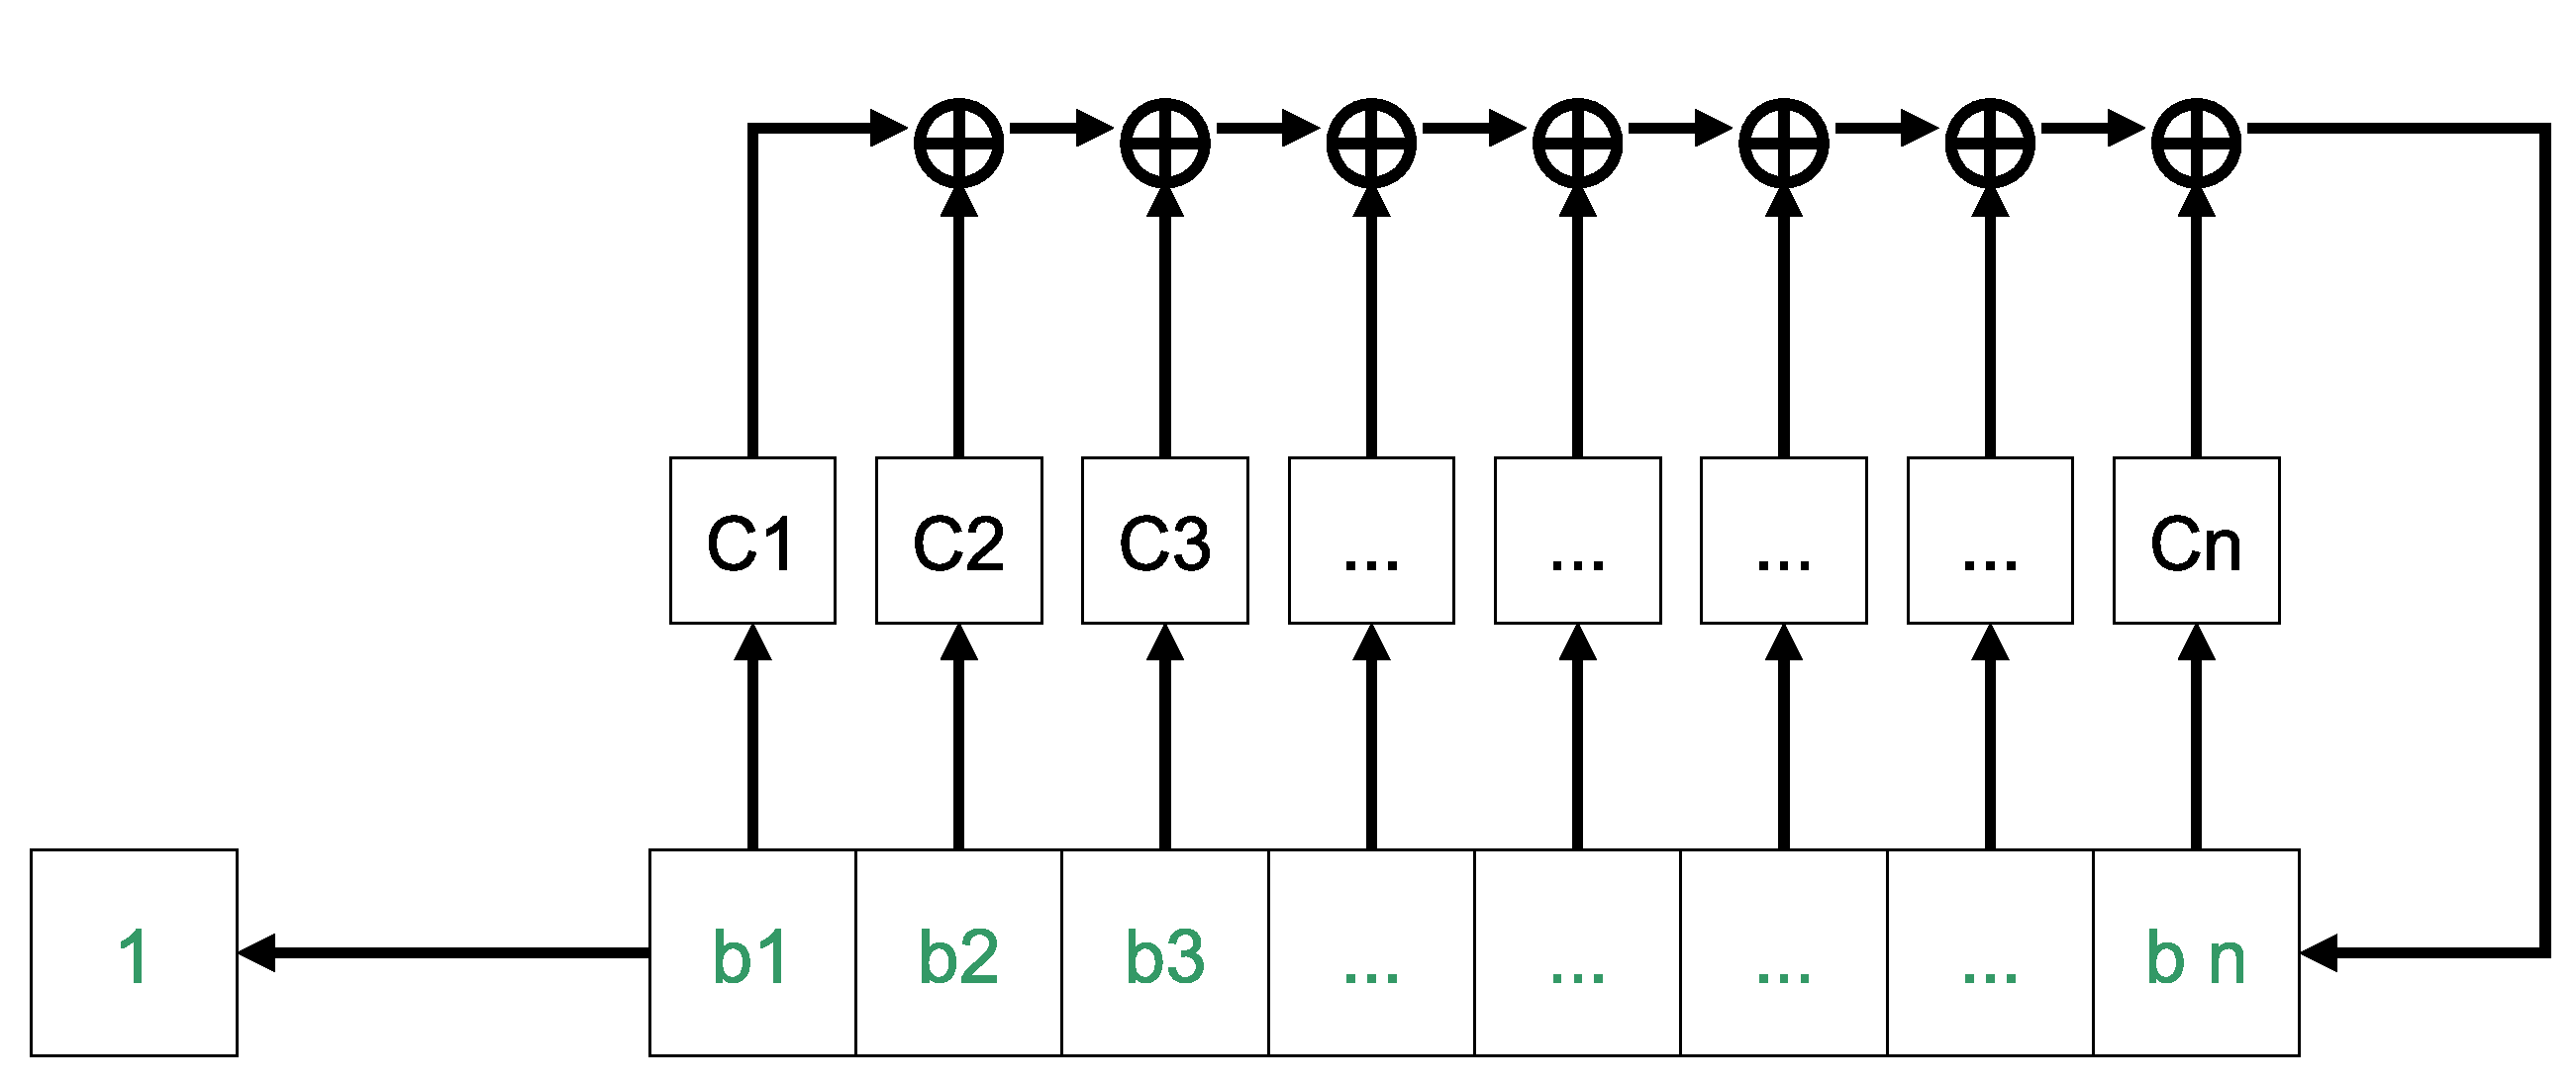
\includegraphics[width=0.75\textwidth]{pic/lfsr}
	\caption{Регистр сдвига с линейной обратной связью}
	\label{fig:lfsr}
\end{figure}

Регистр сдвига состоит из $n$ однобитовых ячеек $b_1, b_2, \dots, b_n$, содержащих 0 или 1, и линейной обратной связи, определяемой коэффициентами $C_1 = 1$, $C_2, C_3, \dots, C_n \in \{0, 1\}$. Многочлен над полем Галуа $GF(2^n)$ вида $C_1 x^n + C_2 x^{n-1} + \dots + C_n x + 1$ называется характеристическим многочленом РСЛОС.

Начальным состоянием генератора является набор значений в битовых ячейках. На каждой итерации генератор вычисляет сумму по модулю два (то есть выполняет операцию XOR) значений ячеек, для которых $C_i=1$:
\[\begin{array}{ll}
	b_{n+1} &= \sum\limits_{i} C_i b_i \mod 2, \\
	b_{n+1} &= b_1 \oplus C_2 b_2 \oplus C_3 b_3 \oplus \dots \oplus C_n b_n.
\end{array}\]

Далее регистр сдвигает значения на одну ячейку влево. Самая правая ячейка $b_n$ принимает вычисленное значение $b_{n+1}$:
\[\begin{array}{ll}
	b_1 & := b_2, \\
	b_2 & := b_3, \\
	\dots \\
	b_n & := b_{n+1}. \\
\end{array}
\]

Выходом генератора является значение ячейки $b_1$ после сдвига.

\example
Пусть регистр сдвига с линейной обратной связью задан характеристическим многочленом $m\left(x\right)=x^{5} + x^{3} + 1$. Как показано на рисунке, регистр состоит из пяти ячеек. В линейной обратной связи будут участвовать ячейки 1 и 3 (то есть $C_1 = 1, C_3 = 1$, остальные $C_i = 0$).

\begin{center}
	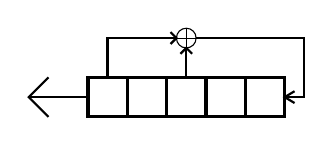
\begin{tikzpicture}[scale=0.05]
		\draw[black,very thick] (30,30) -- (30,40) -- (40,40) -- (40,30) -- (30,30) -- (30,40);
		\draw[black,thick] (35,40) -- (35,50) -- (35,50) -- (37.5,50);
		\draw[black,very thick] (40,30) -- (40,40) -- (50,40) -- (50,30) -- (40,30) -- (40,40);
		\draw[black,very thick] (50,30) -- (50,40) -- (60,40) -- (60,30) -- (50,30) -- (50,40);
		\draw[black,thick] (55,40) -- (55,47.5);
		\draw[black,thick] (53.5,46) -- (55,47.5) -- (56.5,46);
		\draw[black,thick] (37.5,50) -- (52.5,50);
		\draw[black,thick] (51,51.5) -- (52.5,50) -- (51,48.5);
		\draw (55,50) circle [radius=2.5];
		\draw[black] (52.5,50) -- (57.5,50);
		\draw[black] (55,47.5) -- (55,52.5);
		\draw[black,very thick] (60,30) -- (60,40) -- (70,40) -- (70,30) -- (60,30) -- (60,40);
		\draw[black,very thick] (70,30) -- (70,40) -- (80,40) -- (80,30) -- (70,30) -- (70,40);
		\draw[black,thick] (57.5,50) -- (85,50) -- (85,35) -- (80,35);
		\draw[black,thick] (82.5,36.5) -- (80,35) -- (82.5,33.5);
		\draw[black,thick] (30,35) -- (15,35);
		\draw[black,thick] (20,30) -- (15,35) -- (20,40);
	\end{tikzpicture}
\end{center}

Если начальное состояние регистра равно $\vec{s_0} = (0, 0, 0, 0, 1)$, то дальнейшие внутренние состояния регистра $s_i$ и выходы генератора $r_i$ равны:

\begin{enumerate}
	\item $b_{n+1} = b_1 \oplus b_3 = 0 \oplus 0 = 0$, $\vec{s_1} = (0, 0, 0, 1, 0)$, $r_1 = b_1 = 0$;
	\item $b_{n+1} = b_1 \oplus b_3 = 0 \oplus 0 = 0$, $\vec{s_2} = (0, 0, 1, 0, 0)$, $r_2 = b_1 = 0$;
	\item $b_{n+1} = b_1 \oplus b_3 = 0 \oplus 1 = 1$, $\vec{s_3} = (0, 1, 0, 0, 1)$, $r_3 = b_1 = 0$;
	\item $b_{n+1} = b_1 \oplus b_3 = 0 \oplus 0 = 0$, $\vec{s_4} = (1, 0, 0, 1, 0)$, $r_4 = b_1 = 1$;
	\item $b_{n+1} = b_1 \oplus b_3 = 1 \oplus 0 = 1$, $\vec{s_5} = (0, 0, 1, 0, 1)$, $r_5 = b_1 = 0$;
	\item $b_{n+1} = b_1 \oplus b_3 = 0 \oplus 1 = 1$, $\vec{s_6} = (0, 1, 0, 1, 1)$, $r_6 = b_1 = 0$;
	\item $b_{n+1} = b_1 \oplus b_3 = 0 \oplus 0 = 0$, $\vec{s_7} = (1, 0, 1, 1, 0)$, $r_7 = b_1 = 1$;
	\item $b_{n+1} = b_1 \oplus b_3 = 1 \oplus 1 = 0$, $\vec{s_8} = (0, 1, 1, 0, 0)$, $r_8 = b_1 = 0$;
	\item и так далее.
\end{enumerate}

\exampleend

Максимальный период последовательности РСЛОС равен $2^n - 1$. Максимум достигается в том и только в том случае, когда характеристический многочлен РСЛОС примитивен. В этом случае РСЛОС называют регистром сдвига максимального периода, а генерируемые им последовательности -- М-последовательностями или же последовательностями максимального периода.

Если известна структура РСЛОС (значения коэффициентов $C_2, \dots, C_n$), то внутреннее состояние генератора можно восстановить по $n$ предыдущим выходам. По $2n$ предыдущим выходам генератора можно восстановить и внутреннее состояние, и структуру генератора. Зная структуру и текущее внутреннее состояние генератора, можно восстановить его предыдущие и следующие выходные значения.


\section[КСГПСЧ]{Криптографически стойкие генераторы псевдослучайных чисел}\index{генератор!криптографически-стойкий}
\selectlanguage{russian}

Итак, просто генератором псевдослучайных чисел мы называем функцию g вида
	\[g: \left\{0, 1\right\}^{n} \to \left\{0, 1\right\}^{q\left(n\right)},\]
вычислимую за полиномиальное время, результатом работы которой является последовательность чисел, обладающая свойствами случайной.

Были рассмотрены два генератора (линейный конгруэнтный генератор в разделе~\ref{section-linear-congruential-generator} и генератор на основе РСЛОС в разделе~\ref{section-lfsr}). Однако они обладают фундаментальными недостатками, которые не дают их использовать в криптографии. Зная определённое число предыдущих значений выхода генератора (и его внутреннее устройство) криптоаналитик имеет возможность предсказать следующие элементы последовательности. Избежать этого можно только увеличением размера внутреннего состояния.

Пусть $b \left( g \right)$ -- число предыдущих бит, которые необходимо знать криптоаналитику для восстановления внутреннего состояния и параметров генератора (и, следовательно, для предсказания дальнейшей последовательности). И для линейного конгруэнтного генератора\footnote{для получения параметров \texttt{a} и \texttt{c}}, и для генератора на основе РСЛОС функция $b (g)$ является линейной функцией от размера внутреннего состояния $size\left( g \right)$ в битах:

\[\begin{array}{l}
	b \left( LCG \right) = 3 \cdot size\left( g \right), \\
	b \left( LFSR \right) = 2 \cdot size\left( g \right). \\
\end{array}\]

То есть если мы решим увеличить размер внутреннего состояния для защиты от криптоаналитика, это приведёт не более чем к линейному росту затрат последнего на необходимые вычисления (сравните это с экспоненциальным ростом затрат криптоаналитика при увеличении размера ключа для блочных шифров). Поэтому для использования в криптографии к генераторам псевдослучайных чисел предъявляются дополнительные требования.

\emph{Криптографически стойким генератором псевдослучайных чисел} будем называть функцию $g$ вида
	\[g: \left\{0, 1\right\}^{n} \to \left\{0, 1\right\}^{q\left(n\right)},\] 
вычислимую за полиномиальное время, результатом работы которой является последовательность чисел, удовлетворяющая тесту на следующий бит: не должно существовать полиномиального алгоритма, который по $k$ битам последовательности будет предсказывать следующий с вероятностью более $1/2$.

В 1982 году Эндрю Яо (\langen{Andrew Chi-Chih Yao},~\cite{Yao:1982}) доказал, что любой генератор, проходящий тест на следующий бит, сможет пройти и любые другие статистические полиномиальные тесты на случайность.

Как и в случае с блочными шифрами, да и с криптографией вообще, под криптографической стойкостью конкретных алгоритмов в 99\% случаев стоит понимать не принципиальное отсутствие, а неизвестность конкретных алгоритмов, которые могут предсказать выход генератора за полиномиальное время. Для тех генераторов, которые считались криптографически стойкими 20 лет назад, сегодня могут уже существовать алгоритмы для предсказания следующего элемента последовательности.

\subsection{Генератор BBS}
\selectlanguage{russian}

Имеются примеры <<хороших>> генераторов, вырабатывающих криптографически стойкие последовательности, например генератор Blum-Blum-Shub (BBS). Алгоритм работы состоит в следующем: выбирают большие (длиной не менее 512 бит) простые числа\index{число!простое} $p, q$, которые при делении на $4$ дают в остатке $3$. Вычисляют $n = p q$, с помощью генератора случайных чисел вырабатывают число $x_{0}$, где $1 \leq x_0 \leq n-1$ и $\gcd(x_0, n) = 1$. Далее проводят следующие вычисления:
\[ \begin{array}{l}
        x_{1} = x_{0}^{2} \mod n,\\
        x_{2} = x_{1}^{2} \mod n,\\
        \dots,\\
        x_{N} = x_{N-1}^{2} \mod n.
\end{array} \]

Для каждого вычисленного значения оставляют один младший разряд. Вычисляют двоичную псевдослучайную последовательность $k_1, k_2, k_3, \dots$ :
\[ \begin{array}{l}
        k_{1} = x_{1} \mod 2,\\
        k_{2} = x_{2} \mod 2,\\
        \dots,\\
        k_{N} = x_{N} \mod 2.
\end{array} \]

Число $a$ называется \emph{квадратичным вычетом} по модулю $n$, если для него существует квадратный корень $b$ (или два корня): $a = b^2 \mod n$. Для $p,q ~=~ 3 \mod 4$ верно утверждение, что квадратичный вычет имеет единственный корень, и операция $x \rightarrow x^2 \mod n$, применённая к элементам множества всех квадратичных вычетов $\set{QR}_n$ по модулю $n$, является перестановкой множества $\set{QR}_n$.

Полученная последовательность квадратичных вычетов $x_1, x_2, x_3, \dots$ -- периодическая с периодом $T < |\set{QR}_n|$. Чтобы её период для случайного $x_0$ с большой вероятностью оказался большим, числа $p,q$ выбирают с условием малого $\gcd(\varphi(p-1), \varphi(q-1))$, где $\varphi(n)$ -- функция Эйлера.

Полученная последовательность ключей является криптографически стойкой. Доказано, что для <<взлома>> (то есть определения следующего символа с вероятностью, большей $\frac{1}{2}$) требуется разложить число $n=pq$ на множители. Разложение числа на множители считается трудной задачей, все известные алгоритмы не являются полиномиальными по $\log_2 n$.

Оказывается, что если вместо одного последнего бита $k_i = x_i \mod 2$ брать $O(\log_2 \log_2 n)$ последних битов рассмотренного выше генератора $x_i$, то полученная последовательность останется криптостойкой.

Большим недостатком генератора BBS является малая скорость генерирования битов.


\section{КСГПСЧ на основе РСЛОС}

Как уже упоминалось ранее, использование РСЛОС в качестве ГПСЧ не является криптографически стойким. Однако можно использовать комбинацию из нескольких регистров сдвига, чтобы в результате получить быстрый, простой (дешёвый) и надёжный (криптографически стойкий) генератор псевдослучайных чисел.

\subsection[Генераторы с несколькими регистрами сдвига]{Генераторы с несколькими регистрами \protect\\ сдвига}
\selectlanguage{russian}

Первый способ улучшения криптографических свойств последовательности состоит в создании композиционных генераторов из нескольких регистров сдвига при определённом способе выбора параметров. Схема такого генератора показана на рис.~\ref{fig:generators}. Здесь $L_i, ~ i = 1, 2, \dots, M$ -- регистры сдвига с линейной обратной связью. Вырабатываемые ими двоичные символы $x_{1,i}, x_{2,i},  \dots, x_{M,i}$ поступают синхронно на устройство преобразования, задаваемое булевой функцией $f(x_{1,i}, x_{2,i}, \dots, x_{M,i})$. В булевой функции аргументы принимают значения $0,1$ и значения функции также $0,1$.

Число ячеек в $i$-м регистре равно $L_{i}$, причём $\gcd(L_i, L_j)=1$ для $i \neq j$, где $\gcd$ -- наибольший общий делитель. Общее число ячеек $L = \sum\limits_{i=1}^M L_i$. Булева функция $f$ должна включать слагаемое по одному из входов, т.~е. $f = \dots + x_i + \dots$, для того чтобы двоичные символы на выходе этой функции были равновероятными. Период этого генератора может достигать величины (немного меньше)
    \[ T \simeq 2^L. \]

\begin{figure}[!ht]
	\centering
	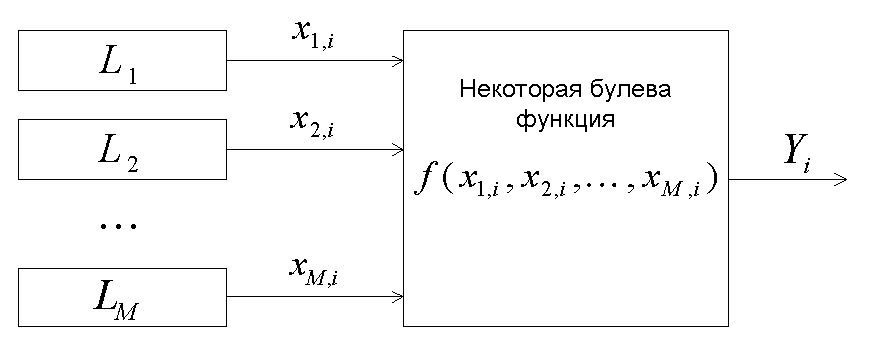
\includegraphics[width=0.7\textwidth]{pic/generators}
    \caption{Генератор с несколькими регистрами сдвига\label{fig:generators}}
\end{figure}

Таким образом, увеличение числа регистров сдвига с обратной связью увеличивает период последовательности. Однако более важным параметром для увеличения криптостойкости генератора является \emph{ длина регистра с линейной обратной связью}, эквивалентного по порождаемой последовательности. Такой эквивалентный регистр с линейной обратной связью находится с помощью алгоритма Берлекэмпа~---~Мэсси декодирования циклических кодов. В лучшем случае длина эквивалентного регистра соизмерима с периодом последовательности, порождённой нелинейным генератором. В общем случае определение эквивалентной длины является сложной задачей.


\subsection[Генераторы с нелинейными преобразованиями]{Генераторы с нелинейными \protect\\ преобразованиями}
\selectlanguage{russian}

Известно, что любая булева функция $f(x_1, x_2, \dots, x_M)$ может быть единственным образом записана многочленом Жегалкина\index{многочлен!Жегалкина}:
\[ \begin{array}{ll}
    f(x_1, x_2, \dots, x_M) & = ~c~ \oplus \\
    & \oplus \sum\limits_{1 \leq i \leq M} c_i x_i \oplus \\
    & \oplus \sum\limits_{1 \leq i < j \leq M} c_{i,j} x_i x_j \oplus \\
    & \oplus \sum\limits_{1 \leq i < j < k \leq M} c_{i,j,k} x_i x_j x_k \oplus \\
    & \oplus \dots \oplus \\
    & \oplus ~ c_{1,2,\dots,M} ~ x_1 x_2 \dots x_M.
\end{array} \]

%Криптографу рекомендуется выбирать булеву функцию с возможно большим числом ненулевых коэффициентов при квадратичных членах полинома Жегалкина.

Второй способ улучшения криптостойкости последовательности поясняется с помощью рис.~\ref{fig:lfsr-zhegalkin}, на котором представлен регистр сдвига с $M$ ячейками и устройство, осуществляющее преобразование с помощью булевой функции $f(x_1, x_2, \dots, x_M)$, причём функция $f$ содержит нелинейные члены, то есть произведения $x_i x_j \dots$. Тактовый вход здесь такой же, как у регистров, показанных на других рисунках.

Если функция $f$ нелинейная, то в общем случае неизвестен полиномиальный алгоритм восстановления состояния регистров по нескольким последним выходам генератора. Таким образом, использование нескольких регистров сдвига увеличивает максимально возможный период по сравнению с одним регистром до $T < 2^{L_1 + L_2 + \dots + L_M}$, а нелинейность функции $f$ позволяет избежать простого нахождения состояния по выходу. Чтобы улучшить криптостойкость последовательности, порождаемой регистром, рекомендуется брать много нелинейных членов многочлена Жегалкина.

Такой подход применён в системе GPS. Удачных попыток её взлома до сих пор нет.

\begin{figure}[!ht]
    \centering
	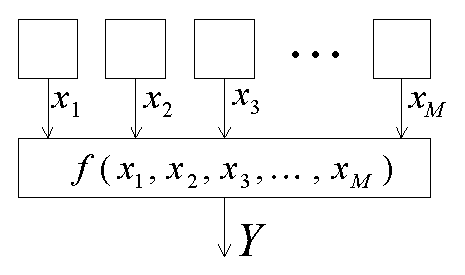
\includegraphics[width=0.4\textwidth]{pic/lfsr-zhegalkin}
    \caption{Криптографический генератор с нелинейной булевой функцией\label{fig:lfsr-zhegalkin}}
\end{figure}


\subsection[Мажоритарные генераторы, шифр A5/1]{Мажоритарные генераторы на примере алгоритма шифрования A5/1}\label{section:majority_generators}\index{шифр!A5}
\selectlanguage{russian}

Третий способ улучшения криптостойкости последовательностей поясняется с помощью рис.~\ref{fig:gsm-a51-cipher}, на котором показан мажоритарный генератор ключей алгоритма потокового шифрования A5/1 стандарта GSM. В отличие от случая нелинейного комбинирования выходов нескольких регистров в этом случае применён условный сдвиг регистров, то есть на каждом такте некоторые регистры могут не сдвигаться, а оставаться в прежнем состоянии. На рисунке показана схема из трёх регистров сдвига с различными многочленами обратной связи (здесь применена обратная нумерация ячеек, коэффициентов и переменных по сравнению с предыдущими разделами):
\[ \left\{ \begin{array}{l}
    c_1(y) = y^{19} + y^{18} + y^{17} + y^{14} + 1, \\
    c_2(y) = y^{22} + y^{21} + 1, \\
    c_3(y) = y^{23} + y^{22} + y^{21} + y^8 + 1.
\end{array} \right. \]

\begin{figure}[!ht]
    \centering
	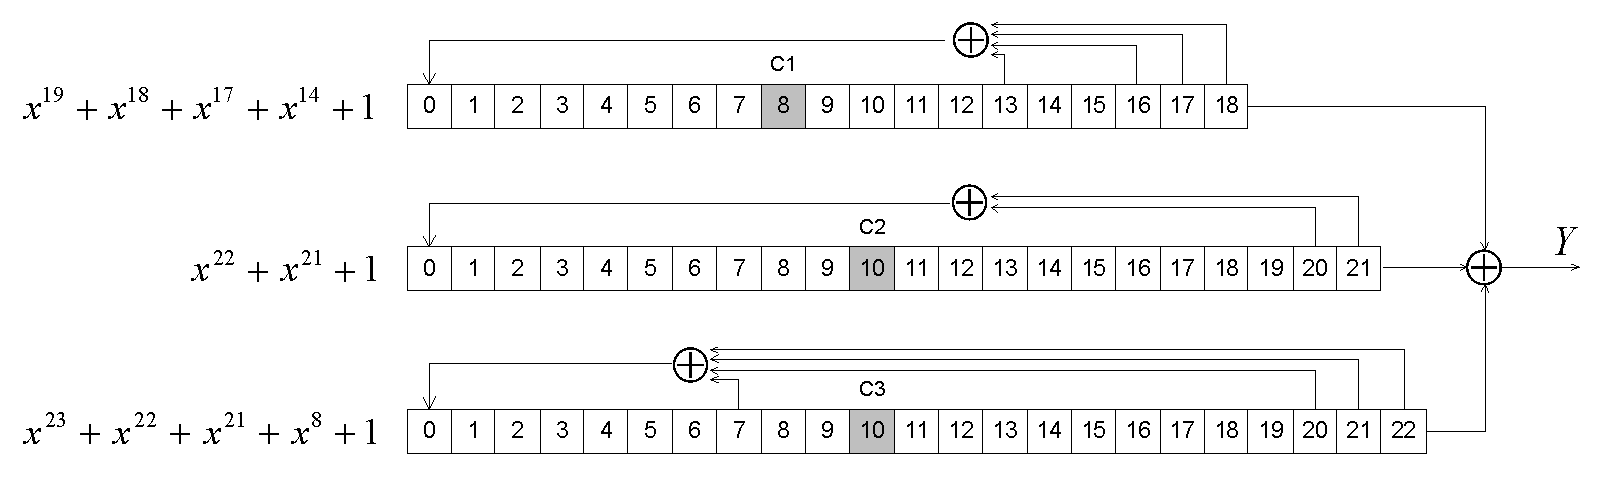
\includegraphics[width=\textwidth]{pic/gsm-a51-cipher}
    \caption{Регистр сдвига алгоритма шифрования A5/1\label{fig:gsm-a51-cipher}}
\end{figure}

В алгоритме A5/1 регистры сдвигаются не на каждом такте. Правило сдвига следующее. В каждом регистре есть один тактовый бит, определяющий сдвиг, -- восьмой бит $\textrm{C1}$ для первого регистра, десятые биты $\textrm{C2}$ и $\textrm{C3}$ для второго и третьего регистров. На каждом такте вычисляется мажоритарное значение тактового бита $m = \textrm{majority}(\textrm{C1}, \textrm{C2}, \textrm{C3})$, то есть по большинству значений: 0 или 1. Если для данного регистра значение тактового бита совпадает с мажоритарным решением, то регистр сдвигается. Если не совпадает, то остаётся в прежнем состоянии без сдвига на следующий такт. Так как всего состояний тактовых битов $2^3$, то в среднем каждый регистр сдвигается в $\frac{3}{4}$ всех тактов.

Общее количество ячеек всех трёх регистров $19+22+23=64$, следовательно, период генератора A5/1: $T < 2^{64}$. Данный шифр не может считаться стойким из-за возможности полного перебора. Например, известны атаки на шифр A5/1, требующие 150-300 GiB оперативной памяти и нескольких минут вычислений одного ПК (2001 г.).

